\section{Existing Solutions Sufficient?}
\label{sec:existing}
In this section, we explore the third question: are existing network-layer solutions sufficient to meet the requirements imposed by the applications in \dis? We start by describing the methodology (\S\ref{ssec:ssmethod}), and then evaluate the network-level (\S\ref{ssec:nlp}) and application-level performance (\S\ref{ssec:alp}) in \dis using existing network-level solutions.

Overall, we conclude that existing transport protocols should be sufficient to handle disaggregated traffic. Specifically, latency-sensitive short memory accesses complete in near-optimal time, while longer flows still experience good performance.

%
\begin{figure}
	\centering
	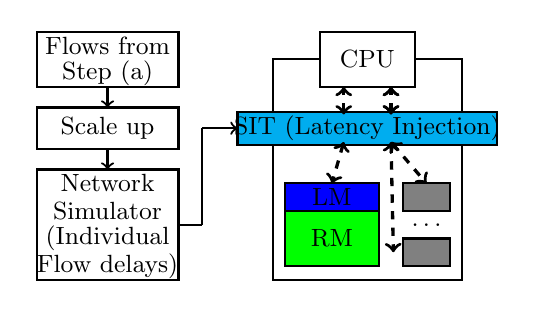
\begin{tikzpicture}[xscale=0.6, yscale=0.35]

	\draw[thick, fill=white] (-8, 5) rectangle (-5, 9); 
	\draw[thick, fill=white] (-8, 9.75) rectangle (-5, 11.25); 
	\draw[thick, fill=white] (-8, 12) rectangle (-5, 14); 
	\draw (-6.5, 8.5) node {\small{Network}};
	\draw (-6.5, 7.5) node {\small{Simulator}};
	\draw (-6.5, 6.5) node {\small{(Individual}};
	\draw (-6.5, 5.5) node {\small{Flow delays)}};
	\draw (-6.5, 10.5) node {\small{Scale up}};
	\draw (-6.5, 13.5) node {\small{Flows from}};
	\draw (-6.5, 12.5) node {\small{Step (a)}};
	\draw[thick, black, ->] (-6.5, 12) -- (-6.5, 11.25);
	\draw[thick, black, ->] (-6.5, 9.75) -- (-6.5, 9);
	\draw[thick, black, -] (-5, 7) -- (-4.5, 7);
	\draw[thick, black, -] (-4.5, 7) -- (-4.5, 10.5);
	\draw[thick, black, ->] (-4.5, 10.5) -- (-3.75, 10.5);

	\draw[thick, fill=white] (-3, 5) rectangle (1, 13); 
	\draw[thick, fill=white] (-2, 14) rectangle (0, 12); 
	\draw (-1, 13) node {\small{CPU}};
	% \draw (-1, 10.5) node {\small{Handler}};
	
	\draw[thick, fill=cyan] (-3.75, 9.9) rectangle (1.75, 11.1); 
	\draw (-1, 10.5) node {\small{SIT (Latency Injection)}};
			
	\draw[thick, fill=blue] (-2.75, 7.5) rectangle (-0.75, 8.5);
	\draw[thick, fill=green] (-2.75, 5.5) rectangle (-0.75, 7.5);
	\draw (-1.75, 8) node {\small{LM}};
%	\draw (-2.75, 7.5) -- (-0.75, 7.5);
	\draw (-1.75, 6.5) node {\small{RM}};
%	\draw (-2.75, 6.5) -- (-0.75, 6.5);
%	\draw (-1.75, 6) node {\small{K$\to$O}};

%	\draw[thick] (-0.25, 5.5) rectangle (0.75, 8.5);
	\draw[thick, fill=gray] (-0.25, 8.5) rectangle (0.75, 7.5);
	\draw[thick, fill=gray] (-0.25, 5.5) rectangle (0.75, 6.5);
	\draw (0.25, 7) node {\small{$\dots$}};

	\draw[very thick, black, dashed, <->] (-1.5, 10) -- (-1.75, 8.5);
	\draw[very thick, black, dashed, <->] (-0.5, 10) -- (0.25, 8.5);
	\draw[very thick, black, dashed, <->] (-0.5, 10) -- (-0.45, 6);

	\draw[very thick, black, dashed, <->] (-1.5, 11) -- (-1.5, 12);
	\draw[very thick, black, dashed, <->] (-0.5, 11) -- (-0.5, 12);
	\draw[very thick, black, dashed, <->] (-0.5, 11) -- (-0.5, 12);

	\end{tikzpicture}
	    \caption{\small{We run real-world applications on a $5$-node Amazon EC2 cluster. To emulate end-to-end network latency, we inject artificial latencies for all ``remote memory'' and ``remote disk'' accesses and measure the impact of this latency to the application-level performance. The latencies injected for each flow are now a result of network simulation results. \rc{SIT representation imprecise}}}
	\label{fig:system3}
\end{figure}
%
\subsection{Methodology}
\label{ssec:ssmethod}
We explore the sufficiency of existing network-layer solutions for \dis in two steps. First, we take the flows generated from \S\ref{sec:workloads} and simulate the network-layer performance (flow completion time) for these flows. We then return to our emulator, take the respective flow completion time for flows, and inject the respective latencies using SIT, as described in \S\ref{sec:requirements}, thus allowing us to evaluate the application level performance. 

For all the simulations in this section, we use the setup from prior work in datacenter transport simulation~\cite{pfabric, phost}. In particular, we simulate a $144$-node full bisection bandwidth fat-tree topology with $40$Gbps access link capacity. \rc{What else do we need to describe?} However, there are multiple challenges in executing the above two steps that we had to resolve.

\paragraphb{Scaling up}
To represent a $144$-node topology using only 13 nodes of measurement data (5 CPU, 5 memory, 3 disk as discussed in \S\ref{sec:methol}), we collected two CDFs representing the interarrival and flow size distributions for each of the 70 possible source-destination pairs (recall from the discussion in \S\ref{sssec:spatialdist} that although there are 13 nodes, certain source-destination pairs will be quiescent). We then assign each node in the topology a sender profile and 12 other nodes in the destination it will send traffic to. We then generate flows between these chosen source-destination pairs by drawing from the appropriate distribution in our traffic matrix. Overall, this method should approximate network traffic in \dis well enough for our evaluation of transport protocols because it draws from our observed distribution of flows that would appear in \dis.
%\begin{enumerate}
%\item our data is for 5 ec2 nodes, but we have a 144-node topology to fill.
%\item the 5 ec2 nodes map to 5 cpu blades, 5 memory blades, and 3 disk blades
%\item so in our 13-node trace we collect a interarrival and size CDF per s-d pair
%\item for each node in the 144, we assign it a sender profile and pick 12 other nodes as destinations
%\item the interarrival and flow size cdfs for flows between a source and destination as picked in the previous step are used to generate flows.
%\item this should give an idea of network loads in a full-dc disaggregated scenario from a transport perspective.
%\end{enumerate}

\paragraphb{Level of disaggregation: $3\times$ problem?}
In a \pdis datacenter network, each node represents a collection of 3 resources --- one unit each of CPU, memory, and disk. Therefore, to represent the same network in a disaggregated context each node should correspond to \emph{three} of a given resource type; that is, one node should contain three units of CPU, memory, or disk. To model this requirement, when generating flows we ran the flow generation scheme described above three times per node.
%\begin{enumerate}
%\item before, one "blade" had 3 resources - cpu, memory, disk
%\item now, each "blade" has only one resource
%\item so, each blade should have 3x of its assigned resource
%\item the flow generation from above is run 3x for each node.
%\end{enumerate}


\subsection{Network-level performance}
Figure~\ref{fig:phostp} shows the performance of pFabric and pHost using the mean slowdown metric, where the flow completion time achieved in simulation for a given flow is normalized by the time it would have taken that flow to complete if it were alone in the network. We observe that for latency-sensitive short flows, the mean slowdown is near-optimal for most applications measured. For longer flows, the performance is slightly worse, but still quite good. \rqc{We conclude that ...}
%\begin{enumerate}
%\item Figure~\ref{fig:phostp} shows network transport performance.
%\item we use the mean slowdown metric used by pFabric and phost~\cite{pfabric, phost}.
%\item the takeaway is that performance is near-optimal for both.
%\item we conclude that existing transport protocols are sufficient because:
%\item \rqc{reasons}
%\end{enumerate}
%\label{ssec:nlp}

%
\begin{figure}
  \centering
%    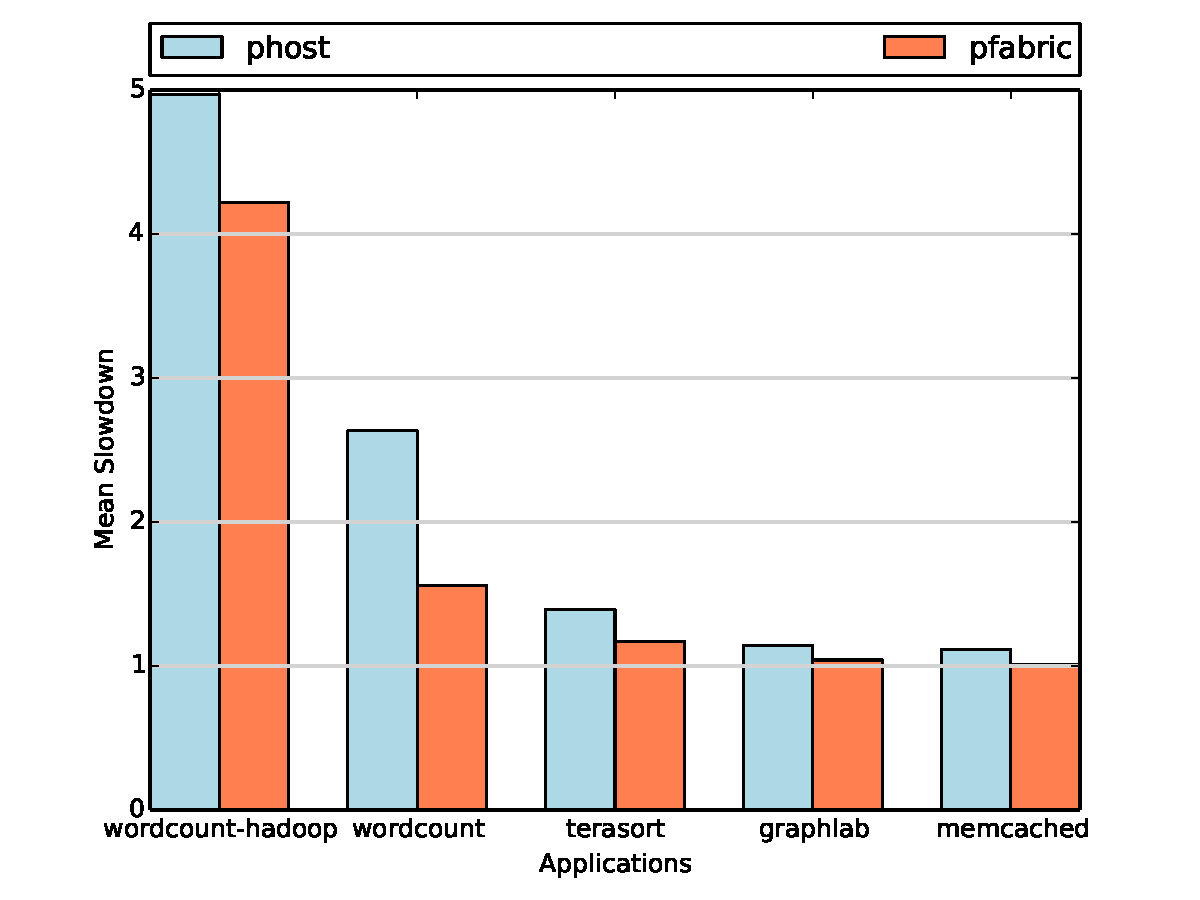
\includegraphics[width = 2.5in]{img/fig12_slowdownsGraph} 
    \subfigure{
    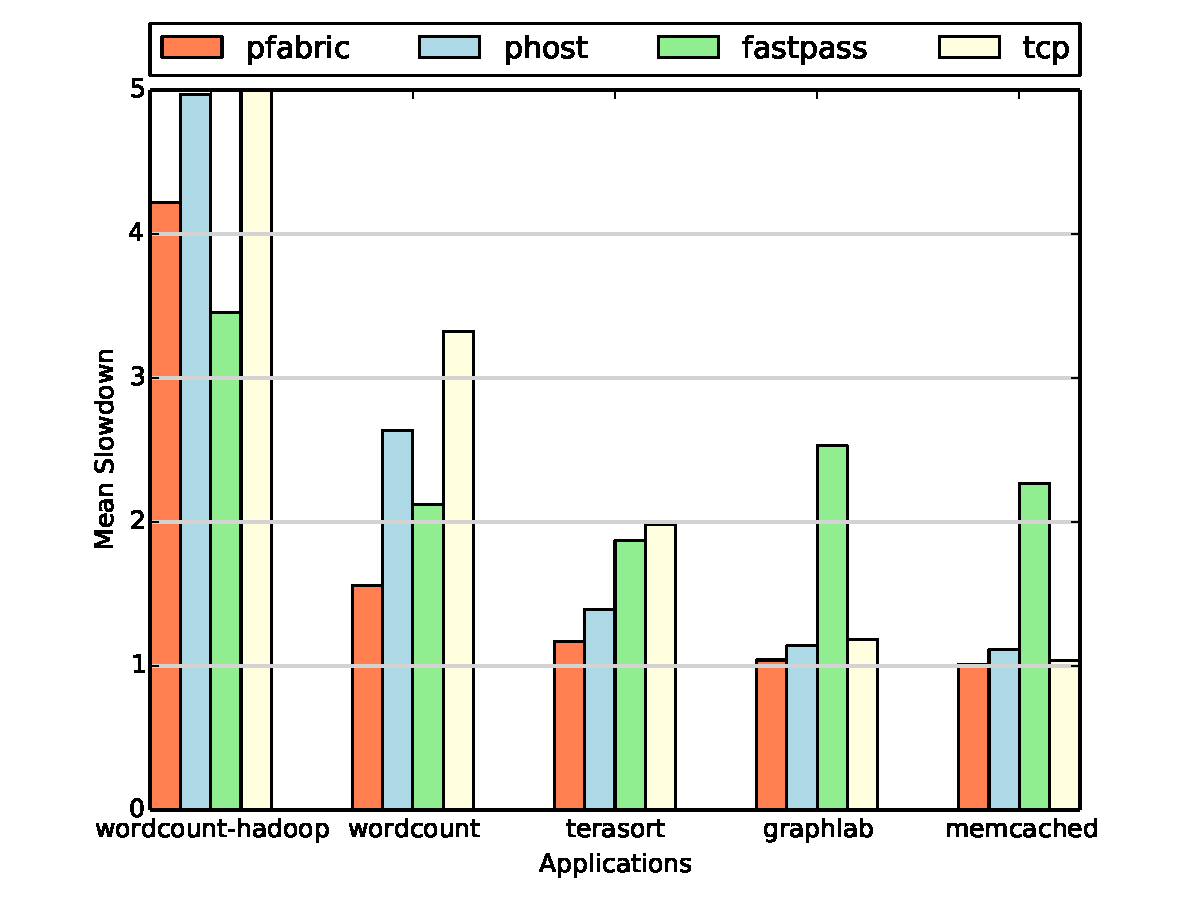
\includegraphics[width=2.5in]{img/fig12_dcScale_slowdownsGraph}
    }
    \subfigure{
    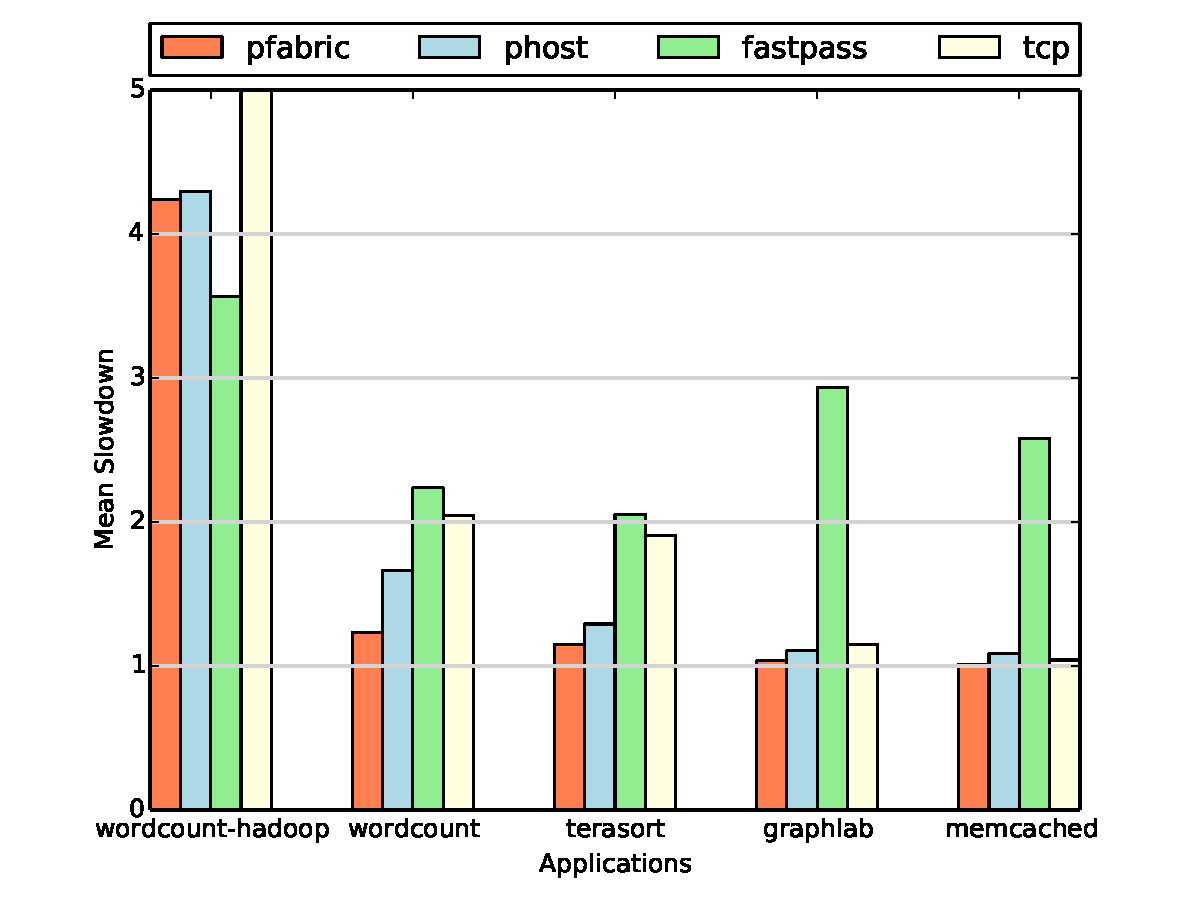
\includegraphics[width=2.5in]{img/fig12_raScale_slowdownsGraph}
    }
  \caption{\small{The mean slowdown for pFabric, pHost, fastpass, and TCP for each of the six applications. Datacenter scale above and rack scale below.}}
  \label{fig:phostp}
\end{figure}
%

\subsection{Application-level performance}
\paragraphb{Latency injection for long flows}
\rqc{need results from peter}

\begin{enumerate}
\item blktrace does not intercept, it only logs
\item we cannot inject latency into disk access
\item this is okay because a. memory is more latency sensitive anyway 
\item and b. there are more memory flows than disk flows.
\item accordingly we only consider the slowdown distribution of memory flows when injecting.
\end{enumerate}
\label{ssec:alp}

%
\begin{figure}
  \centering
    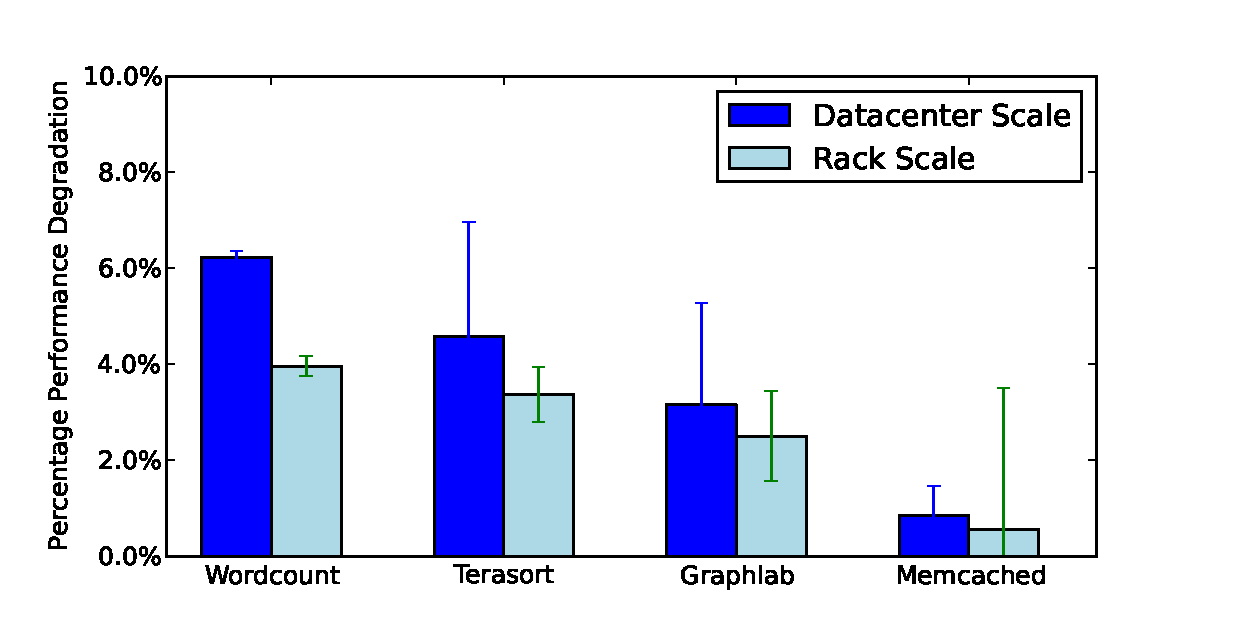
\includegraphics[width = 2.5in]{img/slowdown.eps} 
  \caption{\small{\rqc{Application layer slowdown for each of the six applications.}}}
  \label{fig:appfabric}
\end{figure}
%
